% !TEX root = ../main.tex
\setcounter{section}{-1}
\section{引言}
	\subsection{问题背景}
		近年来随着制造业生产运输及物流业仓储物流等产业的快速发展,由计算机数控机床(Computer Number Controller,CNC)及轨道式智能引导车(Rail Guide Vehicle,RGV)等构成的智能加工系统逐渐成为主流,大大提高了生产效率。考虑到现代生产中生产周期短、生产批次多、生产车间情况复杂的特点,研究智能引导车动态调度模型、优化任务分配制度是有现实意义的。
		\par\indent 图\ref{智能加工系统示意图}是某一个智能加工系统的示意图,由8台CNC、一辆RGV、一条上料传送带、一条下料传送带组成,RGV有一条机械手臂、两只机械手爪以及物料清洗槽,能够完成上料、下料以及清洗物料等多种任务。
		\begin{figure}[htbp]
			\centering
			\caption{智能加工系统示意图}
			\label{智能加工系统示意图}
			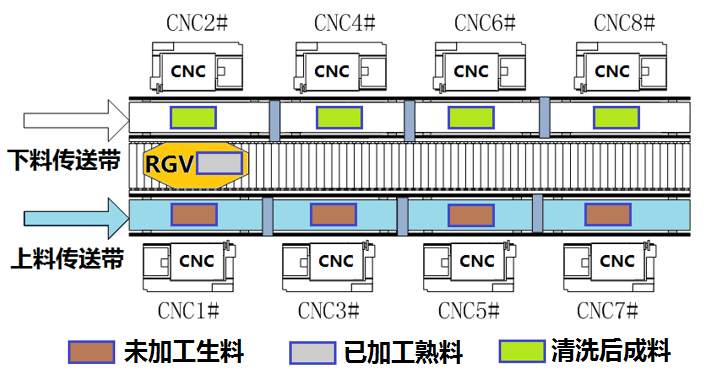
\includegraphics[width=12cm]{machine.png}
		\end{figure}
	\subsection{问题信息}
		\begin{enumerate}
			\item 加工过程包括生料由一道或两道加工工序成为熟料,熟料经过清洗后获得成料;
			\item 一道工序的物料加工作业情况,每台CNC安装同样的刀具,物料可以在任一台CNC上加工完成;
			\item 两道工序的物料加工作业情况,每个物料的第一和第二道工序必须由两台不同的CNC依次加工完成,且加工过程中不能换刀,只能完成一道工序;
			\item CNC在加工过程中可能发生故障且故障的发生概率约为1\%,,故障时未完成物料报废,每次故障排除时间介于\(10\sim20\)分钟之间,故障排除后即刻加入作业序列。且要分别考虑一道工序和两道工序的物料加工作业情况;
			\item RGV同一时间只能执行移动、停止等待、上下料和清洗作业中的一项;
			\item 初始时RGV在CNC1\#和CNC2\#正中间,所有CNC都处于空闲状态;
			\item 传送带运动方向固定,既能联动,也能独立运动,与RGV运输及上料动作同步,保证生料始终及时在等待加工任务的CNC正前方供RGV上料作业;
			\item RGV完成一次上下料后进行熟料清洗作业。清洗作业包括取出槽中成料、放入熟料、将成料放置到下料传送带,清洗作业中RGV不能移动;
			\item 时间单位为秒,班次连续作业时间为8h;
				\begin{table}[htbp]
					\centering
					\caption{智能加工系统作业参数的3组数据表}
					\label{智能加工系统作业参数的3组数据表}
					\begin{longtabu}to\linewidth{@{}X[6,l]|*3{X[c]}@{}}
						\toprule
						系统作业参数                          & 第1组 & 第2组 & 第3组 \\ \midrule
						RGV移动1个单位所需时间                   & 20  & 23  & 18  \\
						RGV移动2个单位所需时间                   & 33  & 41  & 32  \\
						RGV移动3个单位所需时间                   & 46  & 59  & 46  \\
						CNC加工完成一个一道工序的物料所需时间            & 560 & 580 & 545 \\
						CNC加工完成一个两道工序物料的第一道工序所需时间       & 400 & 280 & 455 \\
						CNC加工完成一个两道工序物料的第二道工序所需时间       & 378 & 500 & 182 \\
						RGV为CNC1\#,3\#,5\#,7\#一次上下料所需时间 & 28  & 30  & 27  \\
						RGV为CNC2\#,4\#,6\#,8\#一次上下料所需时间 & 31  & 35  & 32  \\
						RGV完成一个物料的清洗作业所需时间              & 25  & 30  & 25  \\ \bottomrule
					\end{longtabu}
				\end{table}
				\newpage
		\end{enumerate}
	\subsection{问题重述}
		针对下面的三种具体情况:
		\begin{enumerate}
			\item 一道工序的物料加工作业情况,每台CNC安装同样的刀具,物料可以在任一台CNC上加工完成;
			\item 两道工序的物料加工作业情况,每个物料的第一和第二道工序分别由两台不同的CNC依次加工完成;
			\item CNC在加工过程中可能发生故障(据统计:故障的发生概率约为1\%)的情况,每次故障排除(人工处理,未完成的物料报废)时间介于\(10\sim20\)分钟之间,故障排除后即刻加入作业序列。要求分别考虑一道工序和两道工序的物料加工作业情况。
		\end{enumerate}
			有如下两项任务:
		\begin{enumerate}
			\item 任务一:对一般问题进行研究,给出RGV动态调度模型和相应的求解算法;
			\item 任务二:利用题目中系统作业参数的3组数据分别检验模型的实用性和算法的有效性,评价RGV的调度策略和系统的作业效率。
		\end{enumerate}
	\subsection{问题分析}
		\begin{enumerate}
			\item 针对任务一,建立调度模型的一般解法。一般解法分为三部分,一是确定调度模型,二是确定多道工序情况时最优CNC分配与分布模型,三是确定故障情况对整体生产影响的模型。
			\par\indent 针对调度模型,考虑到加工系统的复杂性与连续作业时间长的特点,直接求解全局最优解运算量过大且不易实现。考虑到排队算法求解速度快、局部搜索能力强,适用于获得局部最优解的可行解集合;启发式算法具有在可行解的基础之上进行全局寻优的能力,因此我们先利用排队算法求取局部最优解的可行解集合,再通过启发式算法对可行解集合进行组合优化获得最终最优解,减小了直接求取最优解的运算量;
			\par\indent 针对最优CNC平台分配与分布模型,有如下优先级原则:
				\begin{enumerate}
					\item 加工工序时间与对应CNC平台分配数量成正比;
					\item CNC平台分配时加工第一道工序的CNC平台相对靠近RGV初始位置。在实际加工系统中CNC数量、工序数量、不同工序加工时间是确定的,依据优先级原则可以减小可行解范围,大大减小了利用禁忌算法获得最优分配以及分布结果的迭代次数。
				\end{enumerate}
			\par\indent 针对故障情况对整体生产影响的模型,分为两部分。一是故障发生,二是故障发生时间。其中故障发生服从独立且参数相同的两点分布,故障发生时间服从独立且参数相同的均匀分布,发生时间的取值范围下界为加工开始时间,上界为加工结束时间。
			\item 针对任务二,首先建立模型实用性与算法有效性的指标,包括成料数量与CNC总计空闲时间,针对一道工序有无故障、两道工序有无故障等四种情况分别利用任务一建立的调度模型和分配分布模型计算成果,给出调度策略与作业效率,并通过成料数量与CNC总计等待时间对模型与算法做出评价。
		\end{enumerate}
